%%
% Please see https://bitbucket.org/rivanvx/beamer/wiki/Home for obtaining beamer.
%%
\documentclass{beamer}
\usepackage{natbib}
\usepackage{graphicx}
\usetheme{Singapore}
\usepackage{subfig}
\usepackage{dcolumn}
\usepackage{hyperref}
\title[] %optional
{Using LDA to Identify Knowledge Capital Risks in Annual Reports}

\author[Pedro Vallocci] % (optional)
{Pedro H. Braz Vallocci\inst{1}}

\institute[UCSC] % (optional)
{
  \inst{1}%
  University of California, Santa Cruz
 }

\newcommand{\ffo}{dicfullmc10thr10defnob40noa0_8_4t}
\newcommand{\ffoiii}{dicfullmc10thr10defnob5noa0_8_3t}
\newcommand{\ffovi}{dicfullmc10thr10defnob5noa0_8_6t}

\newcommand{\insertfigurenoffo}[3]{
\begin{figure}[h!]
  \centering
  \includegraphics[width=#3\textwidth]{#1}
  \caption{#2}
  \label{fig:#1}
\end{figure}
}

\newcommand{\insertfigure}[2]{
\begin{figure}[h!]
  \centering
  \includegraphics[width=0.6\textwidth]{\ffo/#1}
  \centering
  \captionsetup{font=scriptsize}
  \caption{#2}
  \label{fig:#1}
\end{figure}
}

\newcommand{\insertfigureiii}[2]{
\begin{figure}[h!]
  \centering
  \includegraphics[width=0.6\textwidth]{\ffoiii/#1}
  \centering
  \captionsetup{font=scriptsize}
  \caption{#2}
  \label{fig:#1}
\end{figure}
}

\newcommand{\insertfigurevi}[2]{
\begin{figure}[h!]
  \centering
  \includegraphics[width=0.6\textwidth]{\ffovi/#1}
  \centering
  \captionsetup{font=scriptsize}
  \caption{#2}
  \label{fig:#1}
\end{figure}
}


\begin{document}
\frame{\titlepage}

\begin{frame}
\frametitle{Outline}
\tableofcontents
\end{frame}

\section{Introduction}
\begin{frame}
\frametitle{Motivation}
\begin{itemize}	
\item \textit{Knowledge capital} represents a firm's cumulative investment in research and development (R\&D) and constitutes a significant portion (38 to 47\%) of its overall value (\cite{Belo2019-iz}).
\item Knowledge capital differs from physical capital in terms of its risk profile:
\begin{itemize}
\item It incurs higher adjustment costs (Belo et al., 2019), experiences greater depreciation (Li et al., 2020), and is subject to factors such as obsolescence and patent breaks.
\end{itemize}
\end{itemize}
\end{frame}

\begin{frame}
\frametitle{Motivation}
\begin{itemize}	
\item Knowledge capital differs from physical capital in terms of its risk profile (2):
\begin{itemize}
\item The cash flow $\theta_t$ in a knowledge-heavy firm can be seen as a stochastic process with innovation jumps: \citep{Andrei2019-bh}  
\begin{equation}
	d \theta_t=\lambda\left(\bar{\mu}-\theta_t\right) d t+\sigma_\theta d W_t^\theta+J d N_t, 
\end{equation}
where $\bar{\mu}$ is the mean profitability, $W_t^\theta$ is a Wiener process, and $J \sim Poisson(f(\Phi))$, where the firm chooses R\&D expenses $\Phi$
\item Do innovation jumps have an effect on stock returns?
\end{itemize}
\end{itemize}
\end{frame}



\begin{frame}
\frametitle{Research question}
  \begin{itemize}
  \item Existing measures are insufficient for identifying knowledge-heavy firms:
\begin{itemize}
\item Inconsistent standards for R\&D reporting across industries and firms, with some firms not disclosing R\&D expenditure in their annual reports.
\item Intangible asset measures done through indirect measures (SG\&A) encompass non-knowledge-related components of organizational capital.
\item Patents only capture the final outcomes of R\&D investment, neglecting the internal learning process within firms.
\end{itemize}
\item Research questions:
\begin{itemize}
\item Can we identify knowledge-heavy firms by performing topic analysis on the risk factors reported in their annual reports?
\item If so, do agents price in different risks for knowledge-heavy firms?
\item More generally, can topic modeling the firms' self-declared risk factor provide a sensible categorization of firms by risk?
\end{itemize}
\end{itemize}
\end{frame}

\begin{frame}
\frametitle{Summary of findings}
\begin{itemize}
	\item Utilizing Latent Dirichlet Allocation (LDA) on a dataset of 10-K risk factors reveals a distinct topic related to knowledge capital risk, referred to as $Topic_{kk}$. %This finding is consistent across various settings, including the analysis with four topics
	\item The ranking of firms based on $Topic_{kk}$ significantly diverges from traditional measures such as accumulated R\&D investments, patent market value, and workforce skills.
	\item  Aligning with existing research, firms with a greater dependency on innovation for generating cash flows exhibit a higher kurtosis in returns. This indicates an elevated tail risk
\end{itemize}
\end{frame}

\begin{frame}
\frametitle{Approach}
\begin{itemize}
\item I employ Latent Dirichlet Allocation (LDA), a topic modeling technique, on a corpus of 121,839 firm annual reports (2006-2022), to identify latent topics.
\item By matching firms based on their CIK and PERMNO, I link the annual reports to daily stock data (aggregated weekly), Compustat data, and measures of firms' knowledge capital, accumulated patent value, and industry skill from existing literature.
%\item I observe a positive association between higher intensities of a specific topic (e.g., "topic kk") and the aforementioned measures. 
\end{itemize}

\end{frame}

\section{Data}


\begin{frame}
\frametitle{Latent Dirichlet Allocation (LDA)}
\begin{itemize}
\small
\item LDA is a generative statistical model widely used for topic modeling in natural language processing (NLP).
\item It operates under the assumption that each document in a corpus is a mixture of a number of latent topics $k \in \{1, ..., K\}$, with weights $\omega_{i1}, ..., \omega_{iK}$. Each topic is assigned a word probability vector $\mathbf{\theta}_k$. 
\item Therefore, if $X_i$ is the vector of word counts with length $n_i$, 
\begin{equation}
X_i \sim \operatorname{Multinomial}\left(n_i, \omega_{i 1} \theta_1+\cdots+\omega_{i K} \theta_K\right)
\end{equation}
\item The output of LDA is a list of topics, each represented as a collection of words, and a weight distribution across these topics for each document.
\end{itemize}
\end{frame}

\begin{frame}
\frametitle{Why LDA?}
\begin{itemize}
\item Other algorithmic text analysis methods used for concept detection include (Ash and Hansen, 2023) dictionary methods, word embeddings, and supervised methods
\item LDA is an unsupervised learning method, meaning that it learns and infers from the data without any predefined labels. Topics generated cannot be targeted towards specific concepts
\item LDA allows for concept exploration without imposing strong priors about the dictionary used and without relying on subjective human labeling, while often creating interpretable topics.
\end{itemize}
\end{frame}

\begin{frame}
  \frametitle{An example of 10-K}
\insertfigurenoffo{apples_1a}{A slice of Apple's 10-K (Item 1A, Risk Factors)}{0.8}
\end{frame}

\begin{frame}
\frametitle{10-K data processing steps}
\begin{figure}[h!]
  \centering
  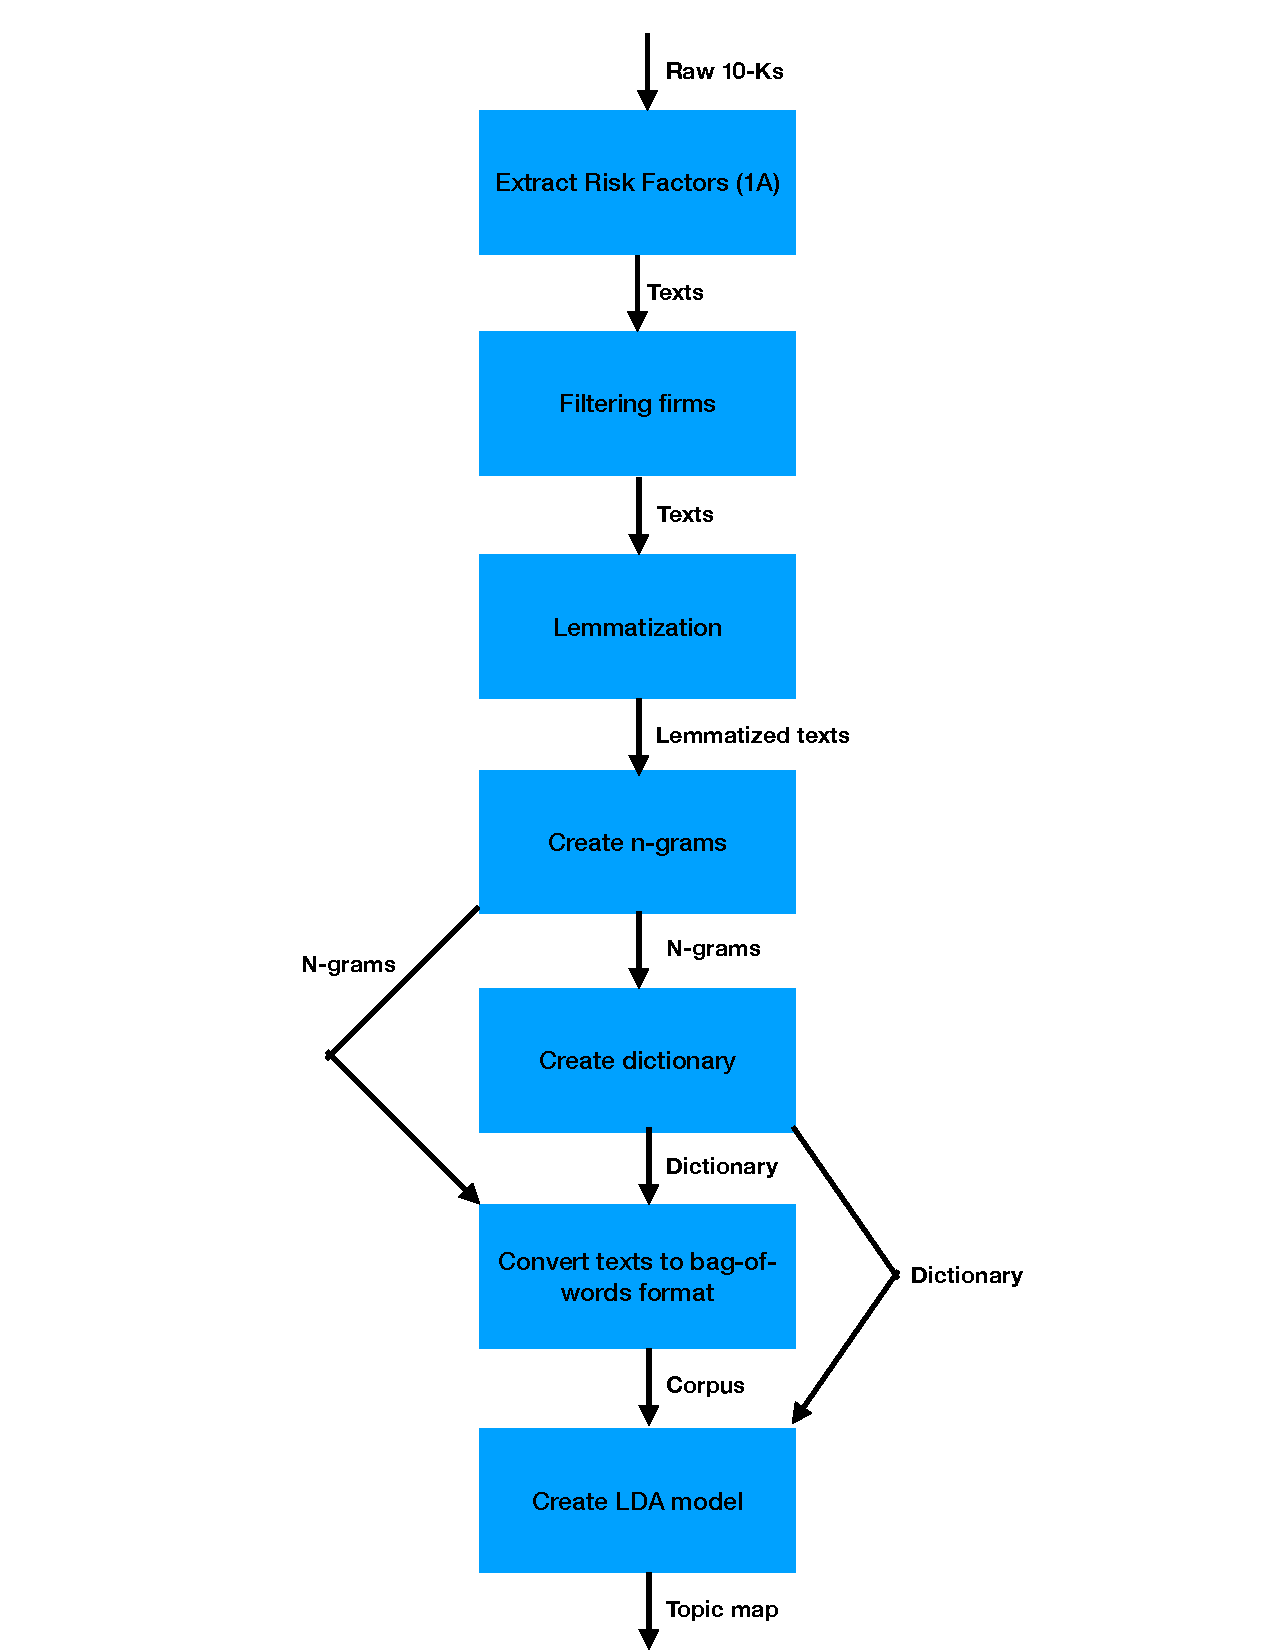
\includegraphics[width=0.5\textwidth]{data_steps.pdf}
  \caption{Data processing steps}
  \label{data_steps}
\end{figure}
\end{frame}

\begin{frame}
\frametitle{Downloading 10-Ks and extracting risk factors}
\begin{itemize}
\item Downloaded from the SEC website 121,839 firm 10-Ks, filed from 2006 to 2022, resulting in approximately 1.6 TB of data. 
\item Extracted the Item 1A (Risk Factors) section from the tree-like structure (XML) of each 10-K.
\item Parsed the text from the Item 1A section using \texttt{BeautifulSoup}; removed punctuation and numbers.
\end{itemize}
\end{frame}


\begin{frame}
\frametitle{Filtering firms (1)}
\begin{itemize}
\item Only ordinary common shares, traded at NYSE, AMEX, or NASDAQ, are kept (\cite{Stambaugh2016-eb}, \cite{Golubov2019-ku}):
\begin{itemize}
  \item I also consider only firms whose stocks were being traded at a minimum price of \$5 in 2016 dollars (\cite{Stambaugh2016-eb})
\end{itemize}
\end{itemize}
\end{frame}



\begin{frame}
\frametitle{Filtering firms (2)}
\begin{itemize}
\item Reporting risk factors is mandatory for most firms, but there are exceptions for asset-backed issuers and smaller reporting companies.
\item Asset-backed issuers are defined as issuers whose reporting obligation arises from the registration of an offering of asset-backed securities under the Securities Act or the registration of a class of asset-backed securities.
\item Firms that are not required to disclose risk factors may leave Item 1A empty or write a placeholder text indicating that they are not required to disclose risk factors due to their nature.
\item This leads to a high frequency of 10-K filings with a significantly low number of words, as shown in Figure \ref{fig:cdf}. In the subsequent stages, 1A texts with an insufficient word count (less than 200 words) are discarded \hyperlink{min_words}{\beamerbutton{Details}}.

\end{itemize}
\end{frame}


\begin{frame}
\frametitle{Filtering firms (4)}
\scriptsize

\begin{table}[!htbp] \centering 

  \label{tab:file_counts} 
\begin{tabular}{@{\extracolsep{5pt}} D{.}{.}{-3} D{.}{.}{-3} D{.}{.}{-3} } 
\\[-1.8ex]\hline 
\hline \\[-1.8ex] 
\multicolumn{1}{c}{Year} & \multicolumn{1}{c}{Total\_1As} & \multicolumn{1}{c}{Filtered} \\ 
\hline \\[-1.8ex] 
\multicolumn{1}{c}{2006} & \multicolumn{1}{c}{5685} & \multicolumn{1}{c}{2466} \\ 
\multicolumn{1}{c}{2007} & \multicolumn{1}{c}{6445} & \multicolumn{1}{c}{2714} \\ 
\multicolumn{1}{c}{2008} & \multicolumn{1}{c}{6931} & \multicolumn{1}{c}{2305} \\ 
\multicolumn{1}{c}{2009} & \multicolumn{1}{c}{8244} & \multicolumn{1}{c}{2190} \\ 
\multicolumn{1}{c}{2010} & \multicolumn{1}{c}{8122} & \multicolumn{1}{c}{2290} \\ 
\multicolumn{1}{c}{2011} & \multicolumn{1}{c}{8019} & \multicolumn{1}{c}{2356} \\ 
\multicolumn{1}{c}{2012} & \multicolumn{1}{c}{7797} & \multicolumn{1}{c}{2316} \\ 
\multicolumn{1}{c}{2013} & \multicolumn{1}{c}{7560} & \multicolumn{1}{c}{2401} \\ 
\multicolumn{1}{c}{2014} & \multicolumn{1}{c}{7560} & \multicolumn{1}{c}{2518} \\ 
\multicolumn{1}{c}{2015} & \multicolumn{1}{c}{7531} & \multicolumn{1}{c}{2528} \\ 
\multicolumn{1}{c}{2016} & \multicolumn{1}{c}{7196} & \multicolumn{1}{c}{2431} \\ 
\multicolumn{1}{c}{2017} & \multicolumn{1}{c}{6896} & \multicolumn{1}{c}{2394} \\ 
\multicolumn{1}{c}{2018} & \multicolumn{1}{c}{6804} & \multicolumn{1}{c}{2418} \\ 
\multicolumn{1}{c}{2019} & \multicolumn{1}{c}{6683} & \multicolumn{1}{c}{2404} \\ 
\multicolumn{1}{c}{2020} & \multicolumn{1}{c}{6531} & \multicolumn{1}{c}{2332} \\ 
\multicolumn{1}{c}{2021} & \multicolumn{1}{c}{6936} & \multicolumn{1}{c}{2308} \\ 
\multicolumn{1}{c}{2022} & \multicolumn{1}{c}{6899} & \multicolumn{1}{c}{1885} \\ 
\hline \\[-1.8ex] 
\end{tabular} 
\caption{The left column shows the count of all 10-Ks retrieved for a given year. The right column counts all the 10-Ks that obey to the following filtering criteria: 1) Ordinary common shares; 2) Membership to NYSE, AMEX, and NASDAQ; 3) Price above \$ 5 in 2006 dollars; 4) Meaningful 10-K contents ($>$ 200 words)} 
\end{table} 

\end{frame}


\begin{frame}
\frametitle{The Process of Lemmatization}
\begin{itemize}
\item Lemmatization is the technique of converting words to their base or root form, effectively eliminating any suffixes and inflections. This ensures semantic consistency across different forms of a word.
\begin{itemize}
  \item For instance, words like "take", "took", and "taken" are all simplified to their common root form, "take".
\end{itemize}
\item The lemmatization process in this project is carried out using the \texttt{spacy} Python library. \texttt{spacy} leverages WordNet, an extensive lexical database of English maintained by Princeton University. 
\end{itemize}
\end{frame}

\begin{frame}
\frametitle{Establishing N-grams and Constructing the Dictionary}
\label{ngram_main}
\begin{itemize}
\item N-grams are defined as groupings of $n$ words appearing together at an unusually high frequency. Examples include phrases like ``New York",``patent application", and `research and development".\hyperlink{ngram_details}{\beamerbutton{Details}}

\item I identified n-grams for $n \leq 3$. For dictionary and bag-of-words purposes, n-grams are treated as distinct words
\item I constructed a dictionary from the ensemble of n-gramized texts. Words were only incorporated into the dictionary if they were featured in a minimum of 0.1\% and less than 80\% of all documents.

\item The final version of my dictionary comprises 24,813 unique words.
\end{itemize}
\normalsize
\end{frame}

\begin{frame}
\frametitle{Conversion of texts to bag-of-words}
\begin{itemize}
\item Using the dictionary and the n-gramized texts, I convert all my texts to a bag-of-words format.
\item The bag-of-words representation ignores the order of words altogether, while keeping the count $c_{ij}$ of appearances of each word $j$ in document $i$, creating the final representation of the \textit{corpus} (\cite{Gentzkow2019-va})
\end{itemize}
\end{frame}

\begin{frame}
\frametitle{Topic modeling}
\begin{itemize}
\item I apply unsupervised topic modeling (Latent Dirichlet Allocation) to the whole corpus of documents containing risk factors for different firm-years, setting as parameter the number \textit{k} of topics, and providing the dictionary previously created.
\begin{itemize}
  \item The choice of \textit{k} is often done \textit{ad hoc} and driven by interpretability (\cite{Gentzkow2019-va})
\end{itemize}
\end{itemize}
\end{frame}

\begin{frame}
	\insertfigure{wordclouds}{Word clouds for each topic in the 4-topic setting. In the following steps, I define $Topic\_kk$ as Topic 3.}
\end{frame}

%\begin{frame}
%  \frametitle{Results}
%  \label{results}
%  \begin{itemize}
%  \item   \href{https://htmlpreview.github.io/?https://github.com/pbrazval/LDA_10Ks/blob/main/dicfullmc10thr10defnob5noa0_8_3t.html}{3-topic model}
%  \item   \href{https://htmlpreview.github.io/?https://github.com/pbrazval/LDA_10Ks/blob/main/dicfullmc10thr10defnob5noa0_8_4t.html}{4-topic model}
%  \item   \href{https://htmlpreview.github.io/?https://github.com/pbrazval/LDA_10Ks/blob/main/dicfullmc10thr10defnob5noa0_8_5t.html}{5-topic model}
%  \item   \href{https://htmlpreview.github.io/?https://github.com/pbrazval/LDA_10Ks/blob/main/dicfullmc10thr10defnob5noa0_8_6t.html}{6-topic model}
%  \item   \href{https://htmlpreview.github.io/?https://github.com/pbrazval/LDA_10Ks/blob/main/dicfullmc10thr10defnob5noa0_8_8t.html}{8-topic model}
%  \item   \href{https://htmlpreview.github.io/?https://github.com/pbrazval/LDA_10Ks/blob/main/dicfullmc10thr10defnob5noa0_8_10t.html}{10-topic model}
%  \item In all these models, knowledge-related words are concentrated in a few topics. 
%  \item Based on the correlation with skill and patent activity in the data, the 4-topic model has provided the best results so far.   \hyperlink{meantiy_details}{\beamerbutton{Mean Topic Intensity by Year}}\hyperlink{robthree}{\beamerbutton{Results with 3 topics}}\hyperlink{robsix}{\beamerbutton{Results with 6 topics}}
%\end{itemize}
%\end{frame}


\begin{frame}
  \frametitle{A sample of the topic map}
The LDA analysis yields a topic map, which assigns topic intensity loadings to each firm-year.
   \tiny
  
\begin{table}[!htbp] \centering 
  \caption{Sample of a topic map} 
  \label{} 
\begin{tabular}{@{\extracolsep{5pt}} D{.}{.}{-3} D{.}{.}{-3} D{.}{.}{-3} D{.}{.}{-3} D{.}{.}{-3} D{.}{.}{-3} } 
\\[-1.8ex]\hline 
\hline \\[-1.8ex] 
\multicolumn{1}{c}{Company\_Name} & \multicolumn{1}{c}{year} & \multicolumn{1}{c}{topic\_0} & \multicolumn{1}{c}{topic\_1} & \multicolumn{1}{c}{topic\_2} & \multicolumn{1}{c}{topic\_3} \\ 
\hline \\[-1.8ex] 
\multicolumn{1}{c}{AEROVIRONMENT INC} & \multicolumn{1}{c}{2010} & \multicolumn{1}{c}{0.822} & \multicolumn{1}{c}{0} & \multicolumn{1}{c}{0.141} & \multicolumn{1}{c}{0.036} \\ 
\multicolumn{1}{c}{AES CORP (THE)} & \multicolumn{1}{c}{2020} & \multicolumn{1}{c}{0.056} & \multicolumn{1}{c}{0.05} & \multicolumn{1}{c}{0.894} & \multicolumn{1}{c}{0} \\ 
\multicolumn{1}{c}{ARROWHEAD PHARMACEUTICALS} & \multicolumn{1}{c}{2016} & \multicolumn{1}{c}{0} & \multicolumn{1}{c}{0} & \multicolumn{1}{c}{0} & \multicolumn{1}{c}{0.997} \\ 
\multicolumn{1}{c}{BROOKDALE SENIOR LIVING INC} & \multicolumn{1}{c}{2015} & \multicolumn{1}{c}{0} & \multicolumn{1}{c}{0.475} & \multicolumn{1}{c}{0.406} & \multicolumn{1}{c}{0.114} \\ 
\multicolumn{1}{c}{ENTERPRISE FINL SERVICES CP} & \multicolumn{1}{c}{2008} & \multicolumn{1}{c}{0} & \multicolumn{1}{c}{0.999} & \multicolumn{1}{c}{0} & \multicolumn{1}{c}{0} \\ 
\multicolumn{1}{c}{II-VI INC} & \multicolumn{1}{c}{2017} & \multicolumn{1}{c}{0.791} & \multicolumn{1}{c}{0.012} & \multicolumn{1}{c}{0.197} & \multicolumn{1}{c}{0} \\ 
\multicolumn{1}{c}{KAISER ALUMINUM CORP} & \multicolumn{1}{c}{2014} & \multicolumn{1}{c}{0.34} & \multicolumn{1}{c}{0.037} & \multicolumn{1}{c}{0.623} & \multicolumn{1}{c}{0} \\ 
\multicolumn{1}{c}{NATURES SUNSHINE PRODS INC} & \multicolumn{1}{c}{2013} & \multicolumn{1}{c}{0.959} & \multicolumn{1}{c}{0} & \multicolumn{1}{c}{0} & \multicolumn{1}{c}{0.04} \\ 
\multicolumn{1}{c}{SOUTHWEST GEORGIA FINL CORP} & \multicolumn{1}{c}{2012} & \multicolumn{1}{c}{0} & \multicolumn{1}{c}{0.999} & \multicolumn{1}{c}{0} & \multicolumn{1}{c}{0} \\ 
\multicolumn{1}{c}{TECO ENERGY INC} & \multicolumn{1}{c}{2006} & \multicolumn{1}{c}{0} & \multicolumn{1}{c}{0} & \multicolumn{1}{c}{0.992} & \multicolumn{1}{c}{0} \\ 
\hline \\[-1.8ex] 
\end{tabular} 
\end{table} 

\end{frame}


\section{Empirical Analysis}

\begin{frame}
\label{defining_kk}
  \frametitle{Defining topic\_kk}
  \begin{itemize}
  \item For every topic map, I follow \cite{Brown2009-zp} and define "topic\_kk" as the topic that has the highest loading within high-tech sectors in the economy, defined as SIC codes 283, 357, 466, 367, 382, 384, 737 (\cite{Brown2009-zp}) 
  
\begin{table}[!htbp] \centering 
  \caption{Topic averages by hi-tech status} 
  \label{fig:bytech} 
\begin{tabular}{@{\extracolsep{5pt}} D{.}{.}{-3} D{.}{.}{-3} D{.}{.}{-3} D{.}{.}{-3} D{.}{.}{-3} } 
\\[-1.8ex]\hline 
\hline \\[-1.8ex] 
\multicolumn{1}{c}{hi\_tech} & \multicolumn{1}{c}{topic\_0} & \multicolumn{1}{c}{topic\_1} & \multicolumn{1}{c}{topic\_2} & \multicolumn{1}{c}{topic\_3} \\ 
\hline \\[-1.8ex] 
\multicolumn{1}{c}{0} & \multicolumn{1}{c}{0.018} & \multicolumn{1}{c}{0.459} & \multicolumn{1}{c}{0.267} & \multicolumn{1}{c}{0.253} \\ 
\multicolumn{1}{c}{1} & \multicolumn{1}{c}{0.308} & \multicolumn{1}{c}{0.584} & \multicolumn{1}{c}{0.02} & \multicolumn{1}{c}{0.086} \\ 
\hline \\[-1.8ex] 
\end{tabular} 
\end{table} 

\end{itemize}
 \end{frame}

\begin{frame}
\frametitle{Topic\_kk vs. patent activity}
       \begin{columns}
          \column{0.6\linewidth}
             \begin{figure}[h!]
		  \centering
		  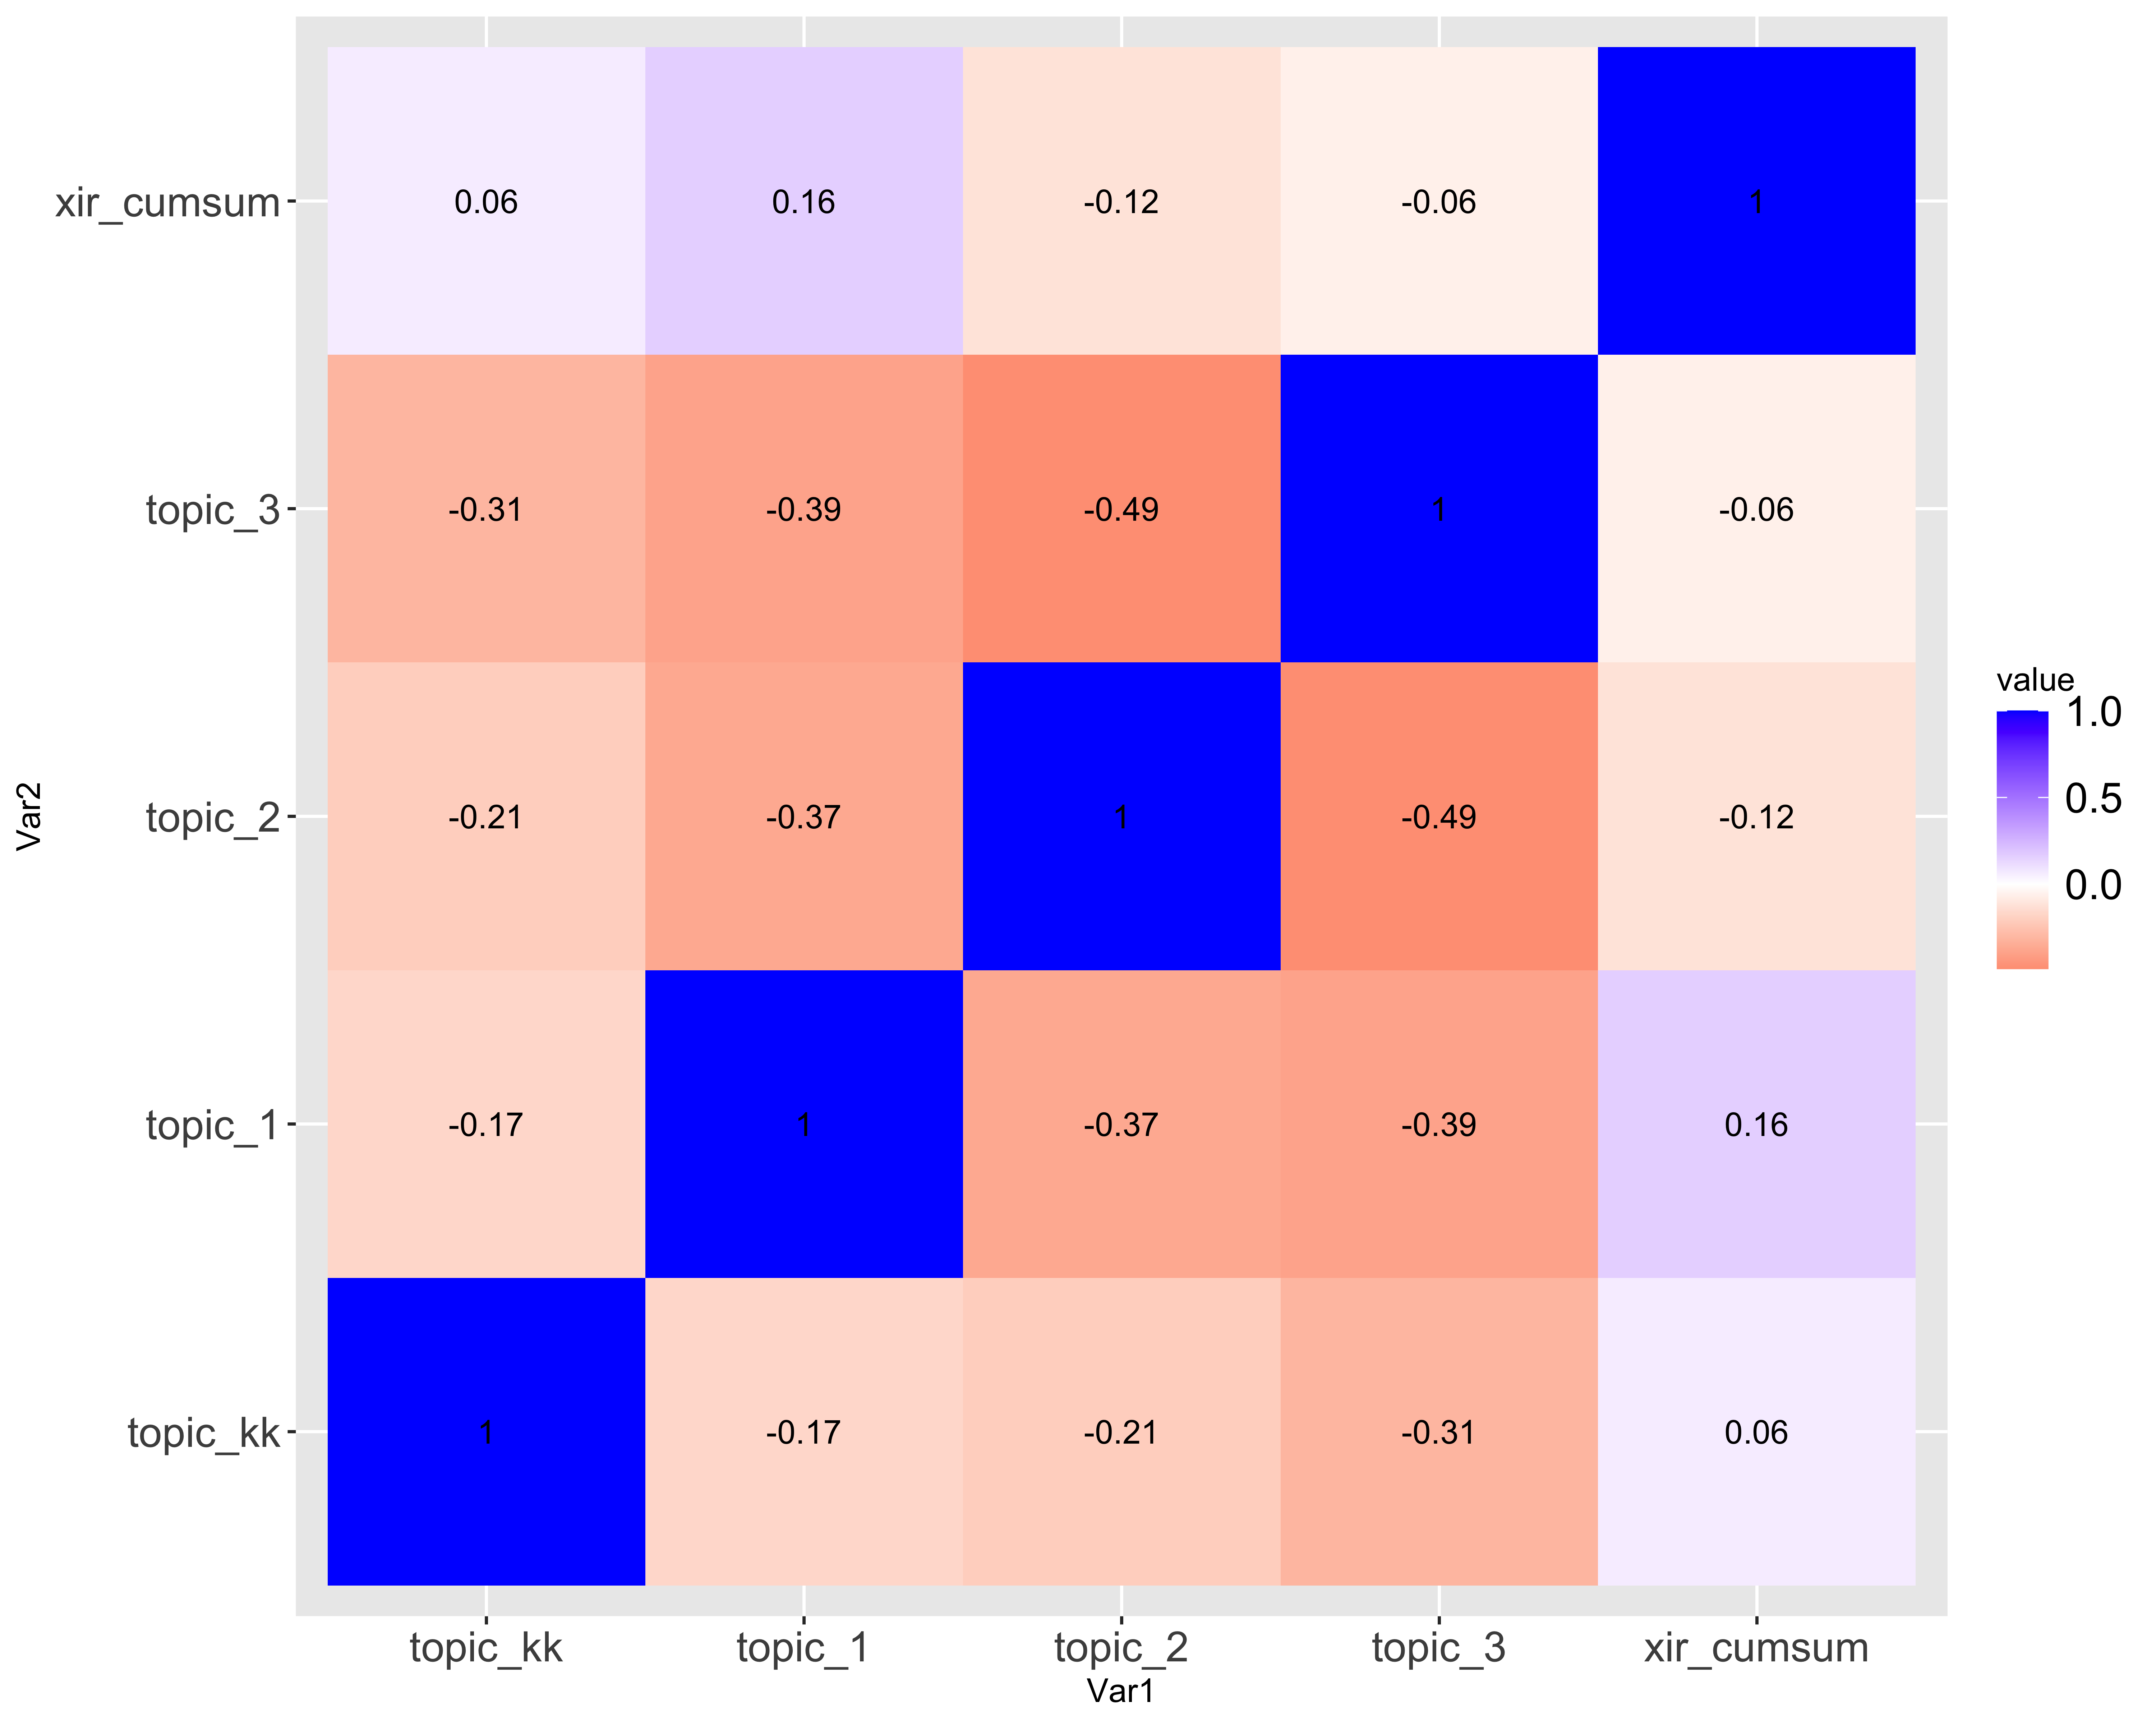
\includegraphics[width=1.2\textwidth]{\ffo/heatmap_patents.png}
		  \captionsetup{font=scriptsize}
		  \label{fig:firmsbypathm}
			\end{figure}
          \column{0.4\linewidth}
          \scriptsize
              \begin{itemize}
              \item Here, I count the co-occurrences of topic\_kk quartiles and accumulated patent-related firm market value.
              \item \cite{Kogan2017-fx} use stock market data to estimate the value of all patents filed by public firms since 1926.
			  \item The vertical axis is divided by yearly defined quartiles of:
			  \begin{equation}
  				\frac{\text{Accumulated Patent Value}}{\text{Total assets}}
				\end{equation}
			  \item A higher accumulated patent value is associated with higher loadings of topic\_kk.
			\end{itemize}
	  \end{columns} 
\end{frame}

\begin{frame}
\frametitle{Topic\_kk vs. Knowledge Capital}
\scriptsize
\insertfigure{topicvskkpt_hm}{Correlation between quartiles of Knowledge capital,  as defined in \cite{Peters2017-fl}, vs. quartiles of topic\_kk. Higher accumulated investments in R\&D are correlated to higher loadings of topic\_kk.}
\end{frame}

\begin{frame}
\frametitle{Topic\_kk vs. Skill}
\scriptsize
\insertfigure{heatmap}{Correlation between different topics and average industry skill, as measured by \cite{Belo2017-qi}. \cite{Belo2017-qi} define industry skill as defined as the share of high-skill workers measured by the BLS; a "high-skill" occupation has Specific Vocational Preparation $\geq 7$ or over two years of preparation.} 
\end{frame}

\begin{frame}
\small 
\frametitle{Pricing knowledge risk premium}
\begin{itemize}
\item To obtain an estimate of knowledge risk premium $\widehat{\lambda}_{kk}$ I analyze firms' weekly returns using a two-stage approach, following \cite{Goyal2012-ct}. 

\item 24 portfolios are formed, expanding \cite{Fama1993-da}. 
\begin{itemize}
	\item Firms are divided into two groups by size, dividing by NYSE's median
	\item Firms are divided into three groups by MB, dividing by NYSE's 30th and 70th percentile
	\item Firms are divided into four groups, according to their quartiles of $topic\_kk$  
\end{itemize}

\item Portfolios are rebalanced every $26^{th}$ calendar-week.
\end{itemize}
\end{frame}

\begin{frame}
\frametitle{Pricing knowledge risk premium}
For each portfolio $i$ and each week $t$, I obtain estimates of betas from the time-series regressions:
	\begin{align*}
		R_{it}-R_{F,t} &= a_i + \beta_{M, i} (R_{M,t}-R_{F,t}) + \beta_{SMB, i} SMB_t \\
		&+\beta_{HML, i} HML_t +\beta_{KKHML, i} KKHML_t \\
		&+\varepsilon_{i,t} 
	\end{align*}
\begin{itemize}
	\item Weekly estimates of $R_{F,t}$, $SMB_t$, $HML_t$ and $R_{M,t}-R_{F,t}$ are retrieved from Kenneth French's website. 
	\item Factor $KKHML_t$ is defined  
\end{itemize}
\end{frame}

\begin{frame}
I then run a cross-sectional regression of average returns on betas:
\begin{align}
\bar{R}_T=\widehat{B} \lambda+\alpha
\end{align}
\end{frame}


\begin{frame}
	\insertfigure{regr}{Results for a sample regression}
\end{frame}

\begin{frame}
\frametitle{Value-weighted returns}
\insertfigure{awawr}{Value-weighted accumulated weekly returns; grouped by quartile of topic\_kk (defined every year). Higher loadings of topic\_kk are associated with higher weekly returns, especially since 2011. }
\end{frame}



\begin{frame}
\frametitle{Value-weighted returns, grouping by topic\_kk (defined for every year-ind12)}
%\insertfigure{awawr_aggind}{Creating topic\_kk quartiles for each year-industry subset, common patterns are less interpretable. I use the 12-industry Fama-French classification.}
\end{frame}

\begin{frame}
\frametitle{Value-weighted returns, grouping by firms' maximum topic}
\insertfigure{awawr_byg}{Value-weighted accumulated weekly returns, grouping by firms' maximum topic. Firms whose topic with maximum loading is topic\_kk (topic 1) has outperformed their peers since 2008.}
\end{frame}

\begin{frame}
\frametitle{Different topics are associated with different cross-sectional volatility patterns}
\insertfigure{wsdr_byg}{Weekly standard deviation of returns within groups, grouped by maximum topic.}
\end{frame}

\begin{frame}
\frametitle{Accumulated assets of firms in the upper quartile of topic\_kk}
\insertfigure{stackedplot_at}{Accumulated assets of firms in the upper quartile of topic\_kk}
\end{frame}



\section{Next Steps}

\begin{frame}
\frametitle{Next steps}
\begin{itemize}
\item This is a work in progress
\item Several moving parts: room for improvement in hyperparameter choice, possibly by cross-validation
\item Test existing benchmarks for choice of $k$ (e.g. perplexity)
\item Move towards supervised models, e.g. by imposing a prior for topic\_kk containing a few words that we expect: e.g. ``patents", ``intellectual property". All the learning so far has been fully unsupervised. 
\item Test whether the created topics can be used as factors in asset pricing models, and if they can explain any anomalies
\item Test whether the language of topic\_kk may have changed over time.
\end{itemize}
\end{frame}

\bibliographystyle{apecon}
\begin{frame}[allowframebreaks]
\frametitle{References}
\bibliography{mylibrary2.bib}
\end{frame}

\section{Appendix}

\begin{frame}
\frametitle{Details of n-gram construction}
\label{ngram_details}
\begin{itemize}
\item n-grams need to appear at least 10 times in the corpus
\item The n-gram must achieve a ``score" of at least 10, using the scoring function from \cite{Mikolov2013-be} \hyperlink{ngram_main}{\beamerbutton{Back to n-gram construction}}
\item I only keep words that have occurred at least 10 times in the whole document; and that are not too common (i.e. that have appeared in 80\% of documents or less)
\end{itemize}
\insertfigurenoffo{mikolov_formula}{Bigram scoring function}{0.3}
\end{frame}

\begin{frame}
\frametitle{Mean Topic Intensity by Year}
\label{meantiy_details}
\hyperlink{results}{\beamerbutton{Back to results}}
\insertfigure{mean_tiy}{Mean Topic Intensity by Year}
\end{frame}


\begin{frame}
\frametitle{Filtering firms (3)}
\label{min_words}
\begin{figure}
  \centering
  \subfloat[Full picture]{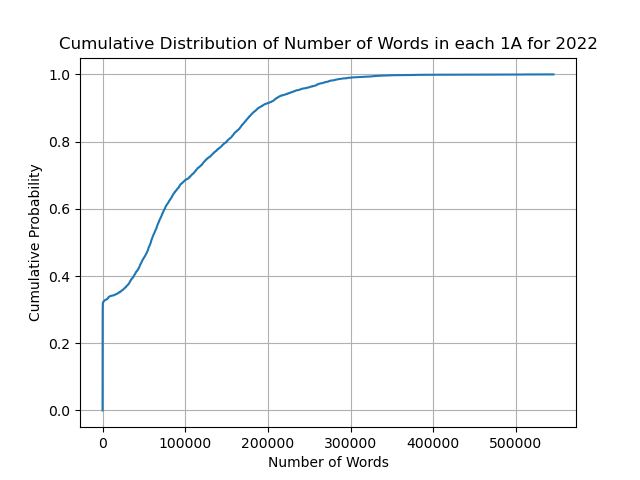
\includegraphics[width=0.45\textwidth]{cdf_words}\label{fig:cdf_words}}
  \hfill
  \subfloat[Detail]{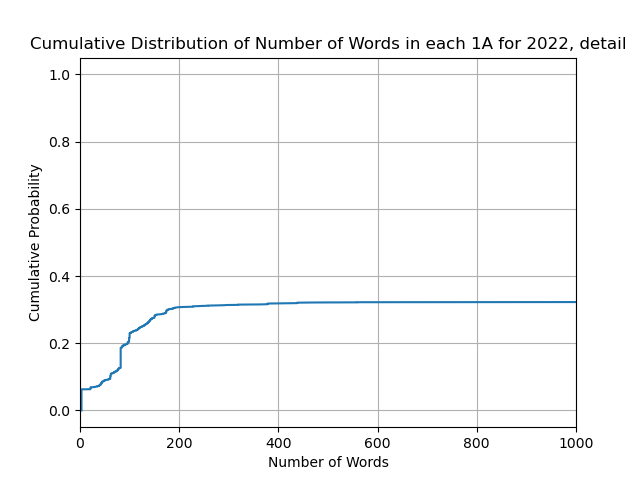
\includegraphics[width=0.45\textwidth]{cdf_words_zoom}\label{fig:cdf_words_zoom}}
  \caption{Word count cumulative distribution function, for all 10-Ks filed in 2022}
  \label{fig:cdf}
\end{figure}
\end{frame}

\begin{frame}
\frametitle{Title}
       \begin{columns}
          \column{0.6\linewidth}
             \begin{figure}[h!]
		  \centering
		  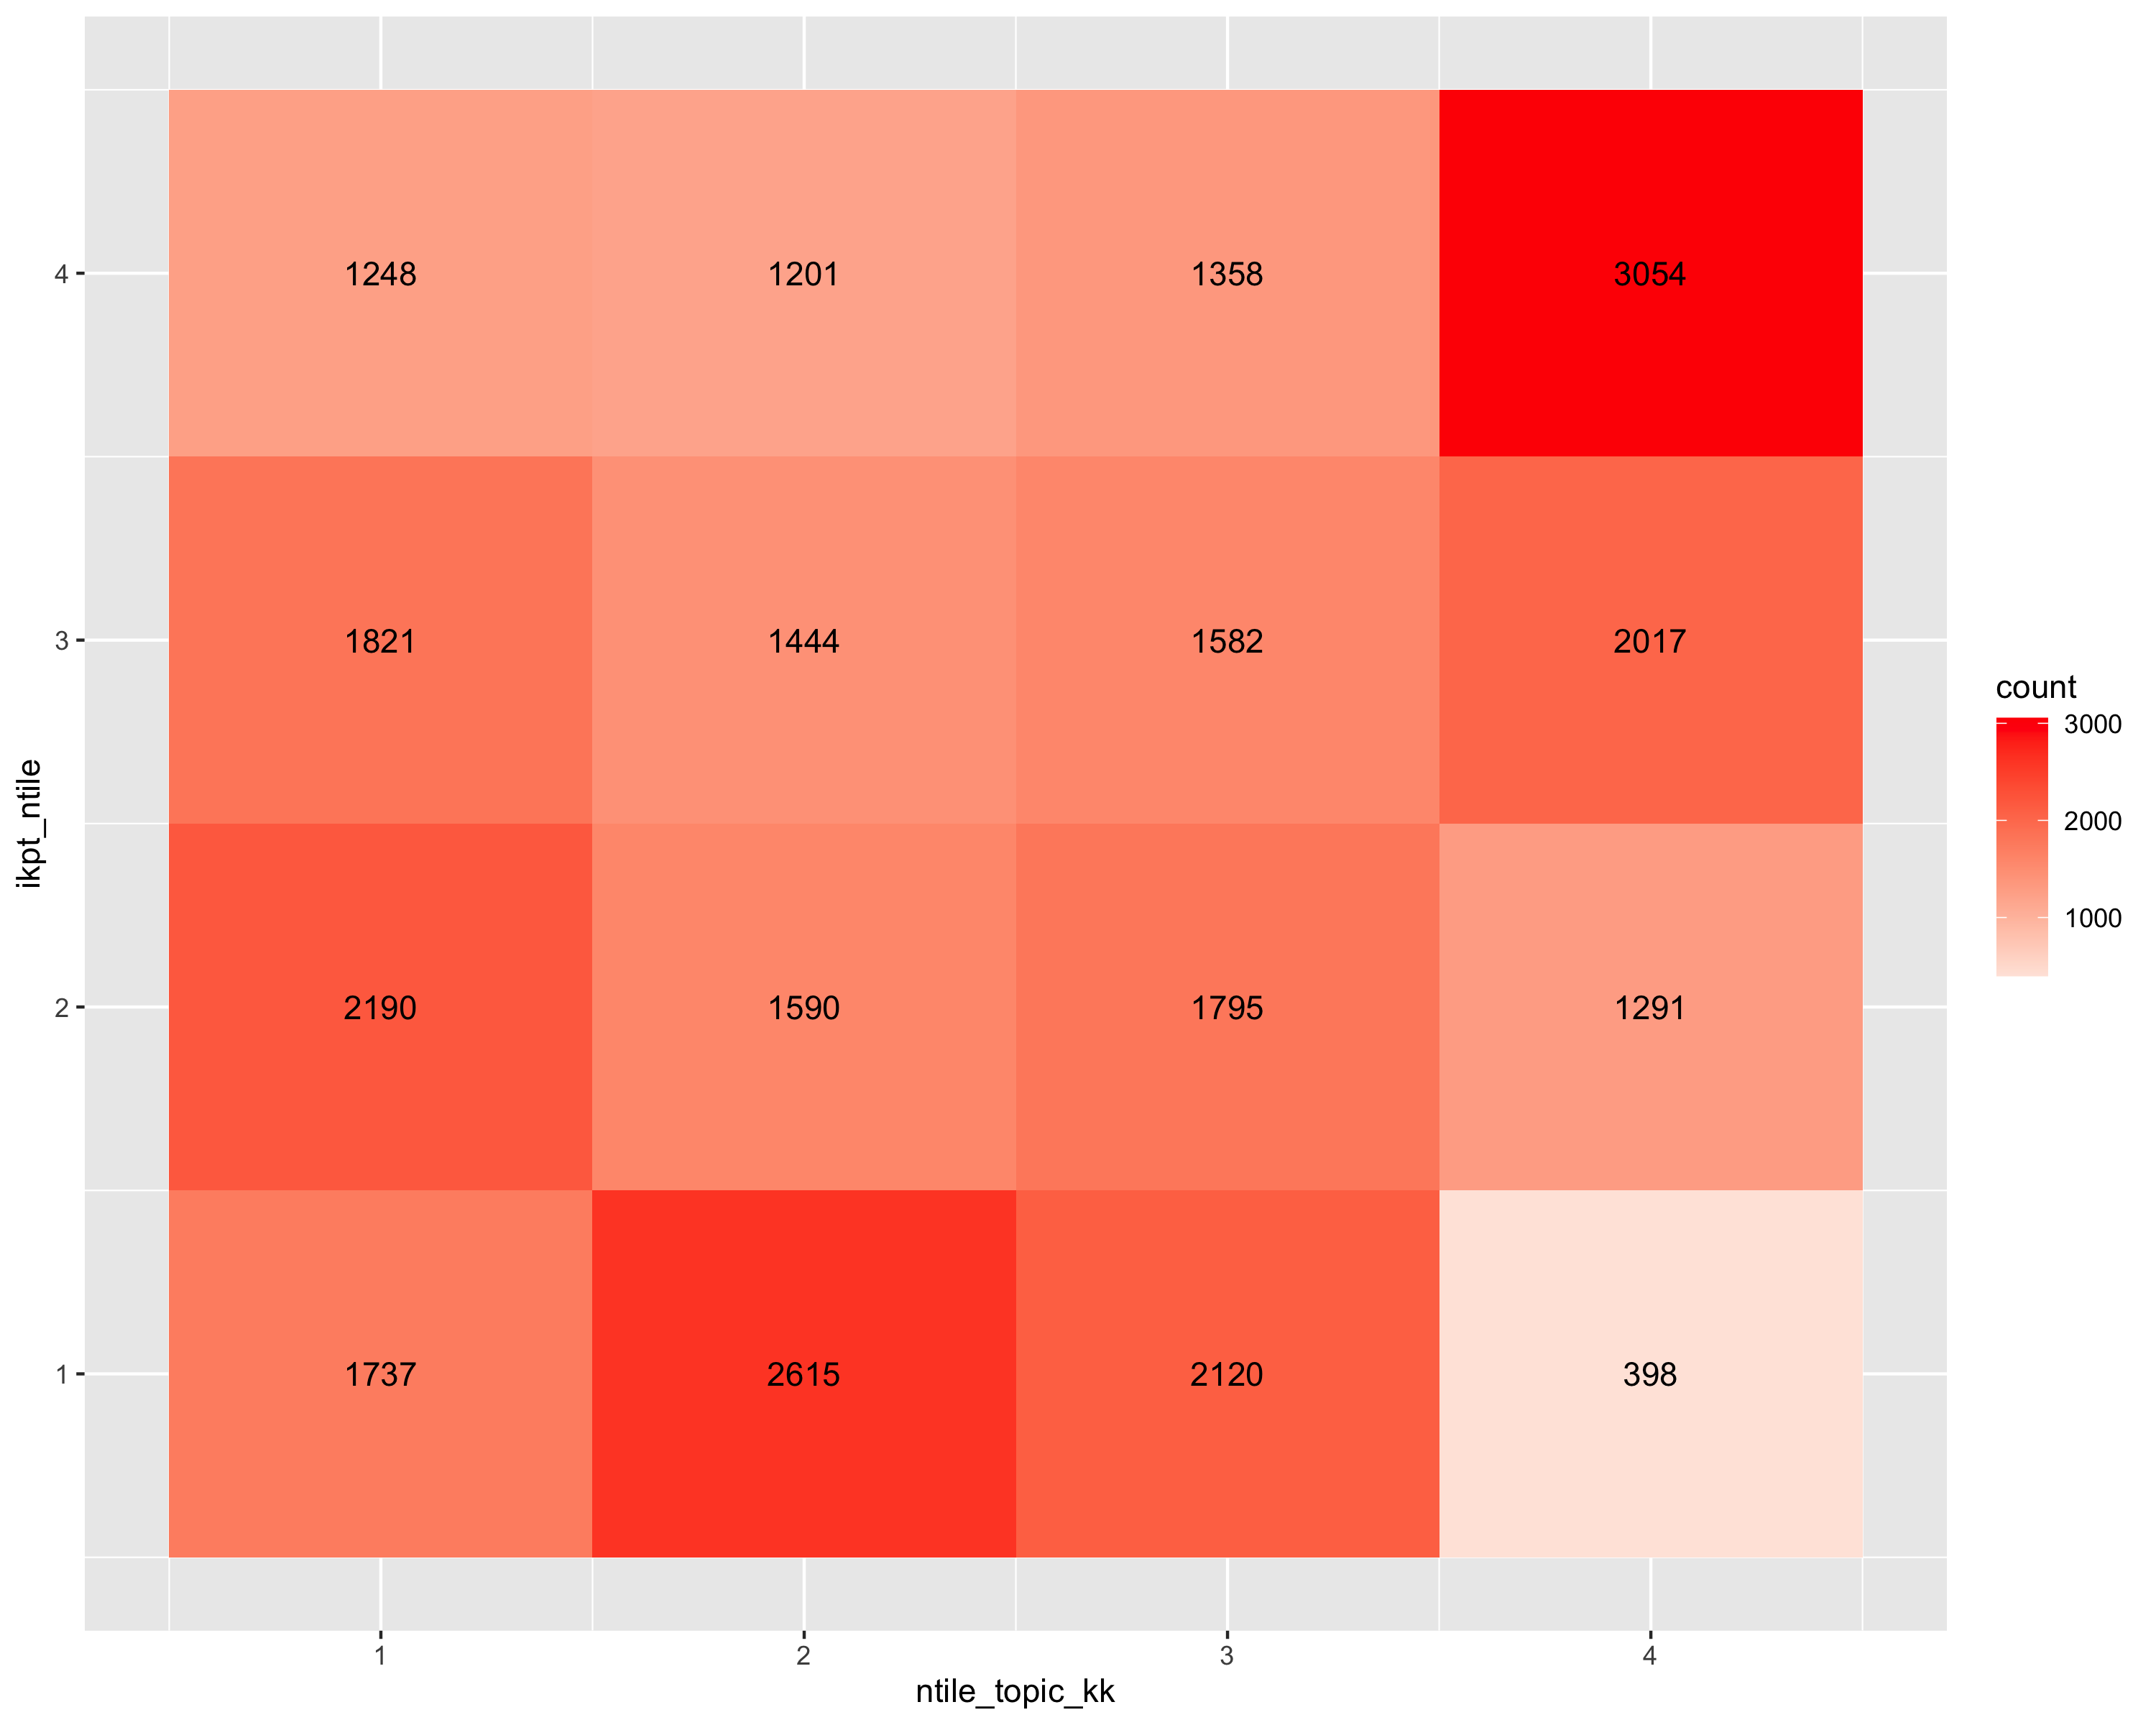
\includegraphics[width=\textwidth]{\ffo/topicvsikpt_hm.png}
		  \centering
		  \captionsetup{font=scriptsize}
		  \label{fig:topicvsikpt_hm}
			\end{figure}
          \column{0.4\linewidth}
          \scriptsize
              \begin{itemize}
			  \item a
			  \item b
			\end{itemize}
	  \end{columns} 
\end{frame}

\begin{frame}
\frametitle{Title}
       \begin{columns}
          \column{0.6\linewidth}
             \begin{figure}[h!]
		  \centering
		  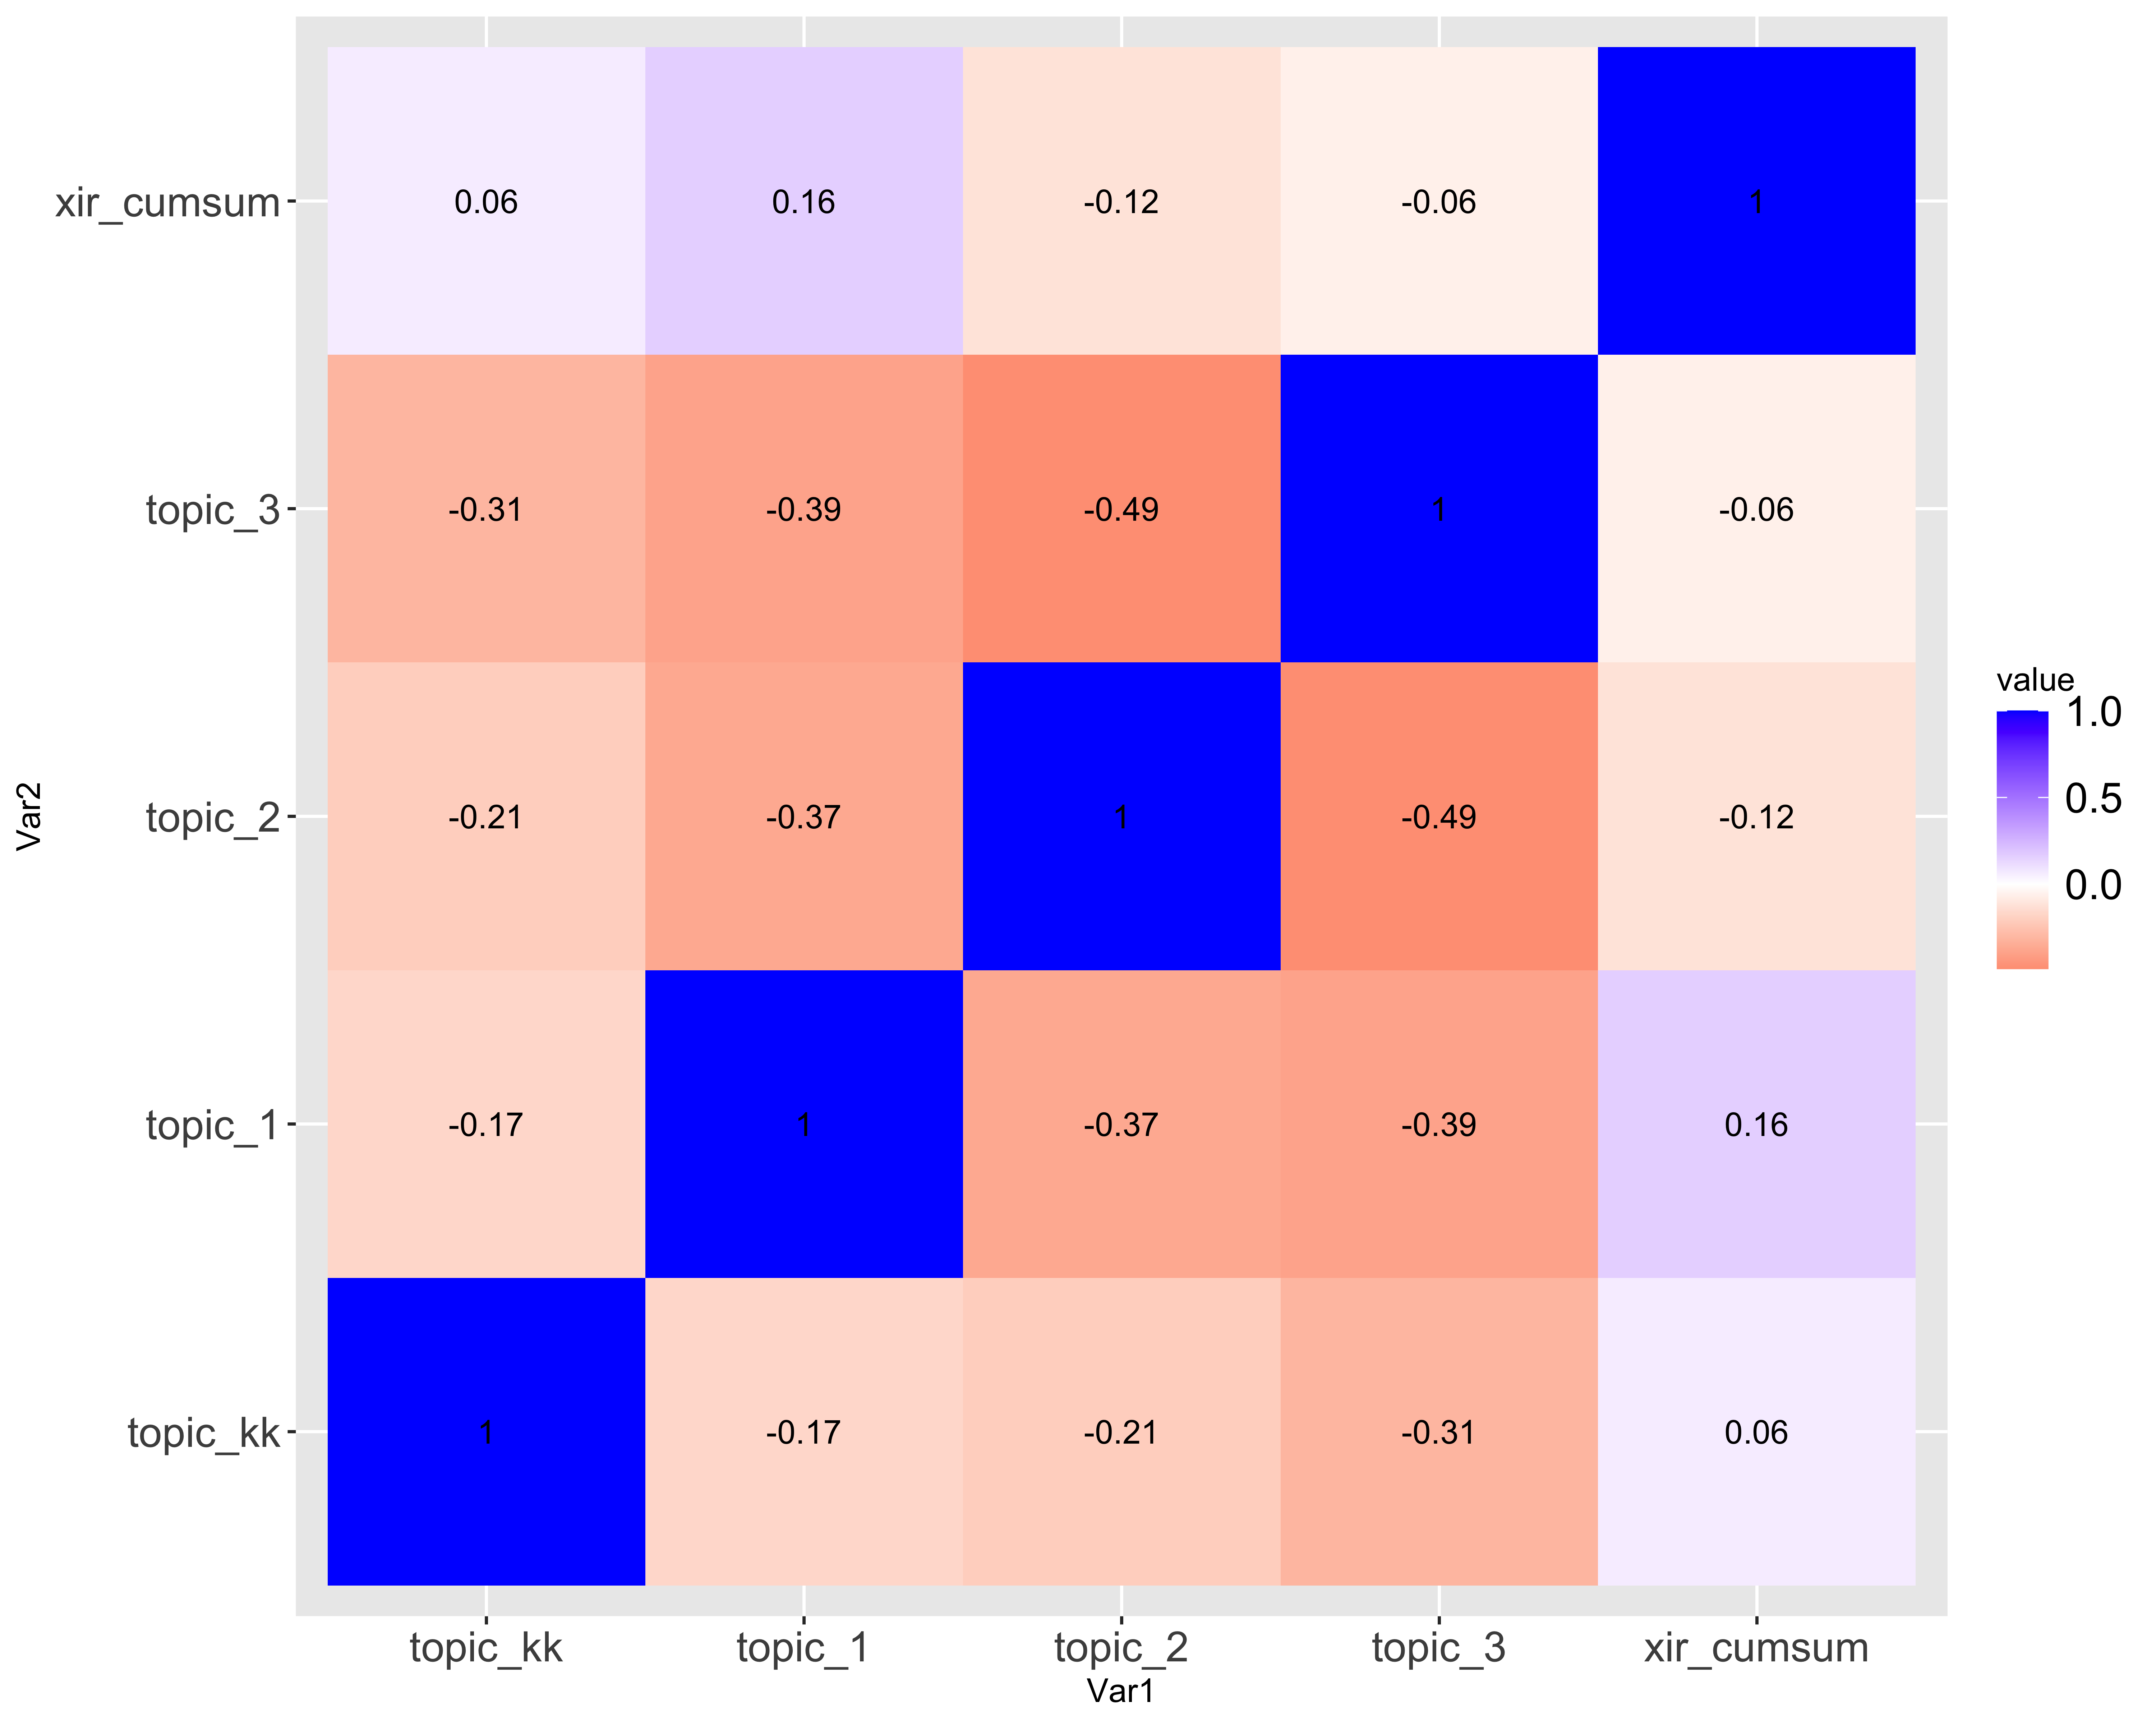
\includegraphics[width=\textwidth]{\ffo/heatmap_patents.png}
		  \captionsetup{font=scriptsize}
		  \label{fig:heatmappatents}
			\end{figure}
          \column{0.4\linewidth}
          \scriptsize
              \begin{itemize}
			  \item a
			  \item b
			\end{itemize}
	  \end{columns} 
\end{frame}

\begin{frame}
\frametitle{Count of firms in the upper quartile of topic\_kk}
\insertfigure{stackedplot_n}{stackedplotn}
\end{frame}

%%%%%%%%%%%%%%%%%%%%%%%%%%%%% ROBUSTNESS TEST: 3 TOPICS
\begin{frame}
\label{robthree}
\centering
\huge\bfseries Robustness tests: 3 topics
\hyperlink{results}{\beamerbutton{Back to results}}
\end{frame}

\begin{frame}
  \frametitle{Defining topic\_kk}
  \begin{itemize}
  \item LDA creates $k$ topics and assigns them to each document of the corpus. "Patents", "intellectual property", and correlated terms tend to be concentrated in few topics.
  \item For every topic map, I define "topic\_kk" as the topic that has the highest loading within high-tech sectors in the economy, defined as SIC codes 283, 357, 466, 367, 382, 384, 737 (\cite{Brown2009-zp}) 
  
\begin{table}[!htbp] \centering 
  \caption{Topic averages by hi-tech status} 
  \label{fig:bytech} 
\begin{tabular}{@{\extracolsep{5pt}} D{.}{.}{-3} D{.}{.}{-3} D{.}{.}{-3} D{.}{.}{-3} D{.}{.}{-3} } 
\\[-1.8ex]\hline 
\hline \\[-1.8ex] 
\multicolumn{1}{c}{hi\_tech} & \multicolumn{1}{c}{topic\_0} & \multicolumn{1}{c}{topic\_1} & \multicolumn{1}{c}{topic\_2} & \multicolumn{1}{c}{topic\_3} \\ 
\hline \\[-1.8ex] 
\multicolumn{1}{c}{0} & \multicolumn{1}{c}{0.018} & \multicolumn{1}{c}{0.459} & \multicolumn{1}{c}{0.267} & \multicolumn{1}{c}{0.253} \\ 
\multicolumn{1}{c}{1} & \multicolumn{1}{c}{0.308} & \multicolumn{1}{c}{0.584} & \multicolumn{1}{c}{0.02} & \multicolumn{1}{c}{0.086} \\ 
\hline \\[-1.8ex] 
\end{tabular} 
\end{table} 

\end{itemize}

\end{frame}


\begin{frame}
\frametitle{Topic\_kk vs. patent activity}
       \begin{columns}
          \column{0.6\linewidth}
             \begin{figure}[h!]
		  \centering
		  \includegraphics[width=\textwidth]{\ffoiii/firmsbypat_hm.png}
		  \captionsetup{font=scriptsize}
		  \label{fig:firmsbypathm}
			\end{figure}
          \column{0.4\linewidth}
          \scriptsize
              \begin{itemize}
              \item Here, I count the co-occurrences of topic\_kk quartiles and accumulated patent-related firm market value.
              \item \cite{Kogan2017-fx} use stock market data to estimate the value of all patents filed by public firms since 1926.
			  \item The vertical axis is divided by yearly defined quartiles of:
			  \begin{equation}
  				\frac{\text{Accumulated Patent Value}}{\text{Total assets}}
				\end{equation}
			  \item A higher accumulated patent value is associated with higher loadings of topic\_kk.
			\end{itemize}
	  \end{columns} 
\end{frame}

\begin{frame}
\frametitle{Topic\_kk vs. Knowledge Capital}
\scriptsize
\insertfigureiii{topicvskkpt_hm}{Correlation between quartiles of Knowledge capital,  as defined in \cite{Peters2017-fl}, vs. quartiles of topic\_kk. Higher accumulated investments in R\&D are correlated to higher loadings of topic\_kk.}
\end{frame}

\begin{frame}
\frametitle{Topic\_kk vs. Skill}
\scriptsize
\insertfigureiii{heatmap}{Correlation between different topics and average industry skill, as measured by \cite{Belo2017-qi}. \cite{Belo2017-qi} define industry skill as defined as the share of high-skill workers measured by the BLS; a "high-skill" occupation has Specific Vocational Preparation $\geq 7$ or over two years of preparation.}. 
\end{frame}

\begin{frame}
\frametitle{Value-weighted returns}

\insertfigureiii{awawr}{Value-weighted accumulated weekly returns; grouped by quartile of topic\_kk (defined every year)}
\end{frame}



\begin{frame}
\frametitle{Value-weighted returns, grouping by topic\_kk (defined for every year-ind12)}
\insertfigureiii{awawr_aggind}{Value-weighted accumulated weekly returns}
\end{frame}

\begin{frame}
\frametitle{Value-weighted returns, defining 4-tiles by year $\times$ ind12}
\insertfigureiii{awawr_byg}{Value-weighted accumulated weekly returns, grouping by firms' maximum topic.}
\end{frame}

\begin{frame}
\frametitle{Different topics are associated with different cross-sectional volatility patterns}
\insertfigureiii{wsdr_byg}{Weekly standard deviation of returns within groups, grouped by maximum topic.}
\end{frame}

\begin{frame}
\frametitle{Accumulated assets of firms in the upper quartile of topic\_kk}
\insertfigureiii{stackedplot_at}{Accumulated assets of firms in the upper quartile of topic\_kk}
\end{frame}


%%%%%%%%%%%%%%%%%%%%%%%%%%%%% ROBUSTNESS TEST: 6 TOPICS
\begin{frame}
\label{robsix}
\centering
\huge\bfseries Robustness tests: 6 topics
\hyperlink{results}{\beamerbutton{Back to results}}
\end{frame}

\begin{frame}
  \frametitle{Defining topic\_kk}
  \begin{itemize}

  \item For every topic map, I define "topic\_kk" as the topic that has the highest loading within high-tech sectors in the economy, defined as SIC codes 283, 357, 466, 367, 382, 384, 737 (\cite{Brown2009-zp}) 
  \tiny
  
\begin{table}[!htbp] \centering 
  \caption{Topic averages by hi-tech status} 
  \label{fig:bytech} 
\begin{tabular}{@{\extracolsep{5pt}} D{.}{.}{-3} D{.}{.}{-3} D{.}{.}{-3} D{.}{.}{-3} D{.}{.}{-3} } 
\\[-1.8ex]\hline 
\hline \\[-1.8ex] 
\multicolumn{1}{c}{hi\_tech} & \multicolumn{1}{c}{topic\_0} & \multicolumn{1}{c}{topic\_1} & \multicolumn{1}{c}{topic\_2} & \multicolumn{1}{c}{topic\_3} \\ 
\hline \\[-1.8ex] 
\multicolumn{1}{c}{0} & \multicolumn{1}{c}{0.018} & \multicolumn{1}{c}{0.459} & \multicolumn{1}{c}{0.267} & \multicolumn{1}{c}{0.253} \\ 
\multicolumn{1}{c}{1} & \multicolumn{1}{c}{0.308} & \multicolumn{1}{c}{0.584} & \multicolumn{1}{c}{0.02} & \multicolumn{1}{c}{0.086} \\ 
\hline \\[-1.8ex] 
\end{tabular} 
\end{table} 

\end{itemize}

\end{frame}


\begin{frame}
\frametitle{Topic\_kk vs. patent activity}
       \begin{columns}
          \column{0.6\linewidth}
             \begin{figure}[h!]
		  \centering
		  \includegraphics[width=\textwidth]{\ffovi/firmsbypat_hm.png}
		  \captionsetup{font=scriptsize}
		  \label{fig:firmsbypathm}
			\end{figure}
          \column{0.4\linewidth}
          \scriptsize
              \begin{itemize}
              \item Here, I count the co-occurrences of topic\_kk quartiles and accumulated patent-related firm market value.
              \item \cite{Kogan2017-fx} use stock market data to estimate the value of all patents filed by public firms since 1926.
			  \item The vertical axis is divided by yearly defined quartiles of:
			  \begin{equation}
  				\frac{\text{Accumulated Patent Value}}{\text{Total assets}}
				\end{equation}
			  \item A higher accumulated patent value is associated with higher loadings of topic\_kk.
			\end{itemize}
	  \end{columns} 
\end{frame}

\begin{frame}
\frametitle{Topic\_kk vs. Knowledge Capital}
\scriptsize
\insertfigurevi{topicvskkpt_hm}{Correlation between quartiles of Knowledge capital,  as defined in \cite{Peters2017-fl}, vs. quartiles of topic\_kk. Higher accumulated investments in R\&D are correlated to higher loadings of topic\_kk.}
\end{frame}

\begin{frame}
\frametitle{Topic\_kk vs. Skill}
\scriptsize
\insertfigurevi{heatmap}{Correlation between different topics and average industry skill, as measured by \cite{Belo2017-qi}. \cite{Belo2017-qi} define industry skill as defined as the share of high-skill workers measured by the BLS; a "high-skill" occupation has Specific Vocational Preparation $\geq 7$ or over two years of preparation.}. 
\end{frame}

\begin{frame}
\frametitle{Value-weighted returns}
\insertfigurevi{awawr}{Value-weighted accumulated weekly returns; grouped by quartile of topic\_kk (defined every year)}
\end{frame}



\begin{frame}
\frametitle{Value-weighted returns, grouping by topic\_kk (defined for every year-ind12)}
\insertfigurevi{awawr_aggind}{Value-weighted accumulated weekly returns}
\end{frame}

\begin{frame}
\frametitle{Value-weighted returns, defining 4-tiles by year $\times$ ind12}
\insertfigurevi{awawr_byg}{Value-weighted accumulated weekly returns, grouping by firms' maximum topic.}
\end{frame}

\begin{frame}
\frametitle{Different topics are associated with different cross-sectional volatility patterns}
\insertfigurevi{wsdr_byg}{Weekly standard deviation of returns within groups, grouped by maximum topic.}
\end{frame}

\begin{frame}
\frametitle{Accumulated assets of firms in the upper quartile of topic\_kk}
\insertfigurevi{stackedplot_at}{Accumulated assets of firms in the upper quartile of topic\_kk}
\end{frame}


\end{document}
